\documentclass{report}
\author{Damian Herman, SKN Teleinformatyki Apacz500, \\ Wydział Elektryczny Zachodniopomorskiego Uniwersytetu Technologicznego \\Katedra przetwarzania sygnałów i inżynierii multimedialnej}
\title{Apacz Laser Tank}
\usepackage[utf8]{inputenc}
\usepackage[T1]{fontenc}
\usepackage{lmodern}
\usepackage{graphicx}
\usepackage[polish]{babel}
\usepackage{indentfirst}
\usepackage{float}
\begin{document}
    
    \maketitle
    \chapter{Wprowadzenie do projektu}
        Apacz Laser Tank jest projektem zdalnie sterowanego pojazdu gąsienicowego opartego początkowo o plaftormę Raspberry Pi 3, a następnie ze względu na rozmiary - 
        Arduino Mini Pro. Sterowanie odbywa się za pomocą wieloplaformowej aplikacji napisanej przy pomocy frameworka Xamarin, pozwalając na uruchomienie aplikacji na urządzeniach 
        z Windows oraz Android. 

        Pojazd jest napędzany dwoma silnikami prądu stałego z przekładniami, sterowanymi przy pomocy mostka H. Komunikacja pomiędzy aplikacją, a pojazdem odbywa się przy pomocy Bluetooth.
        Projekt jest udostępniony w serwisie Github, na licencji MIT.
    \chapter{Instalacja}
        \section{Wymagania}
            Instalacja projektu wymaga środowiska programistycznego Visual Studio 2017 w wersji przynajmniej Community. Wersja Express środowiska \textbf{nie zadziała}.  
            Dodatkowo, wymagane jest zainstalowanie edytora Arduino IDE albo samego WinAVR. Zamiast Arduino IDE można użyć edytora Visual Studio Code/VSCodium z wtyczką PlatformIO.
            Aby aplikacja na Androida uruchomiła się, wymagany jest smartfon z wersją 6.0 Nougat lub wyższą, a w wypadku aplikacji UWP na plaftormę Windows 10 - wymagana jest aktualizacja Creator's Update.
        \subsection{Proces instalacji}
        Kod źródłowy aplikacji Xamarin oraz firmware Arduino jest dostępne są tutaj: https://github.com/Alienwaren/Apacz500-Laser-Tank pod postacią repozytorium git.
        Aby uzystkać dostęp do kodu wystarczy sklonować repozytorium przy pomocy polecenia \textit{git clone https://github.com/Alienwaren/Apacz500-Laser-Tank}
        \subsubsection{Visual Studio Community 2017}
        Ze strony visualstudio.com należy pobrać instalator środowiska VS Community, a następnie go uruchomić. W nowym oknie zaznaczyć następujące opcje:
        \begin{enumerate}
            \item Opracowywanie zawartości dla plaftormy uniwersalnej systemu Windows
            \item Programowanie aplikacji klasycznych dla plaformy .NET
            \item Opracowywanie aplikacji mobilnych za pomocą środowiska .NET
        \end{enumerate}
    	\begin{figure}[H]
    		\centering
    		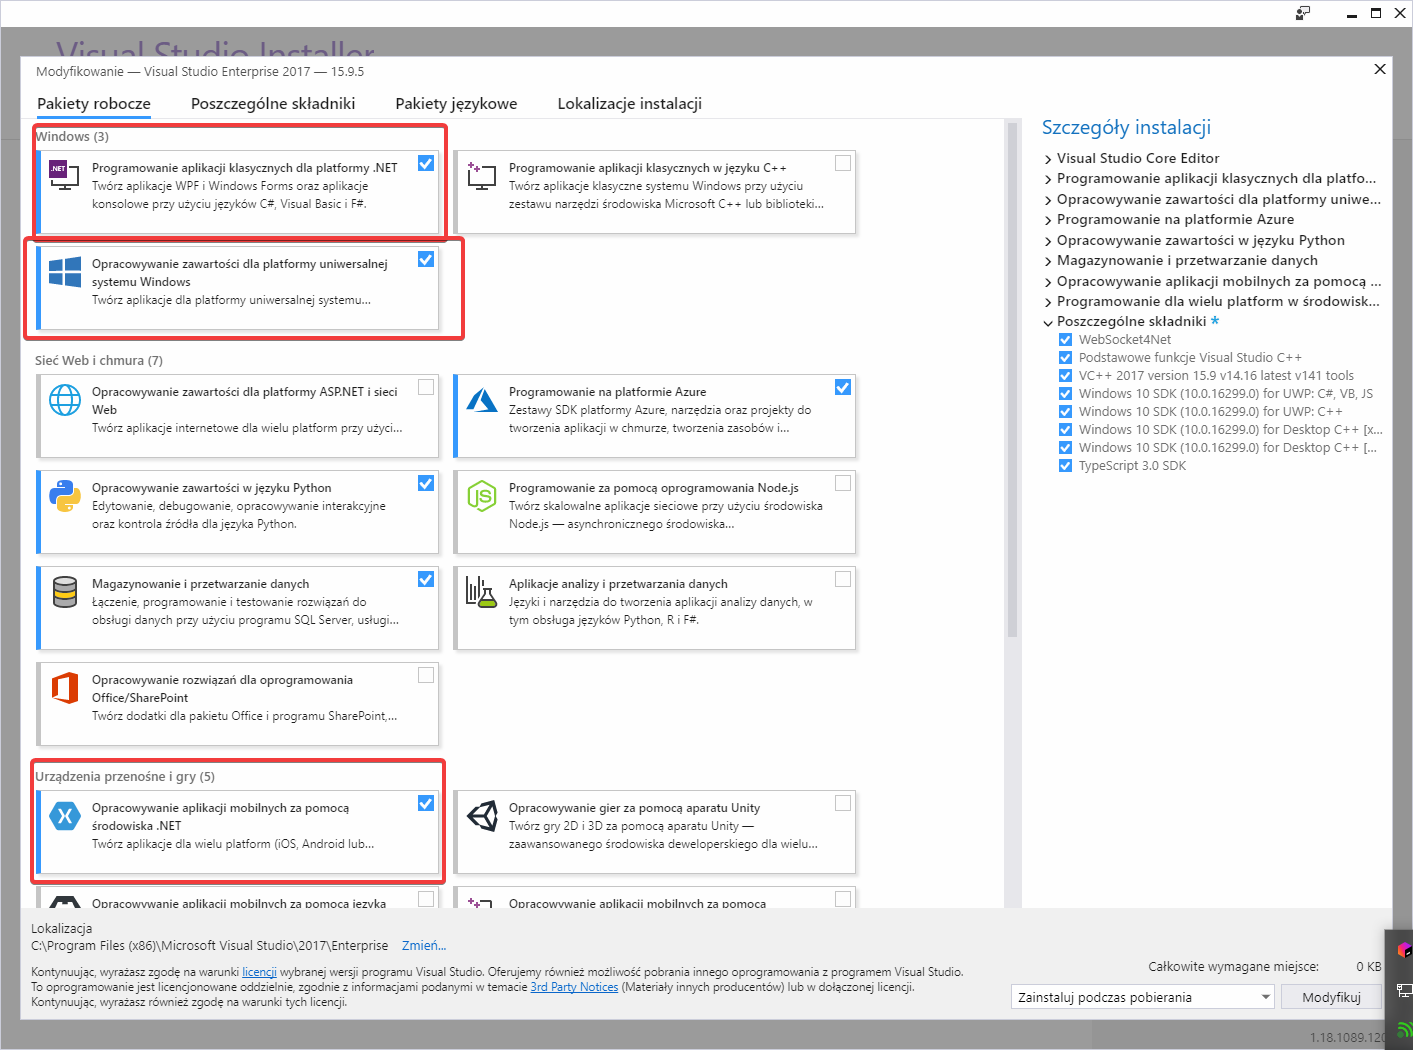
\includegraphics[scale=0.3]{visual_1.png}
    		\caption{Okno instalatora Visual Studio, z zaznaczonymi zależnościami potrzebnymi do używania projektu}
    	\end{figure}
        Po zatwierdzeniu instalacji, program pobierze i zainstaluje potrzebne komponenty.
        \subsubsection{Platform IO}
		Zamiast Arduino IDE wykorzystano Platform IO, ponieważ oferuje lepsze wsparcie dla pisania kodu - podpowiedzi składni, wsparcie dla wielu platform embedded oraz integracja z git. Platform IO jest wydawany w postaci wtyczki do Visual Studio Code/VSCodium oraz edytora Atom. 
		
		Aby zainstalować wtyczkę do Visual Studio Code (zakładając, że edytor jest już zainstalowany), należy uruchomić edytor a następnie kliknąć na odpowiednią ikonę.
		
		\begin{figure}[H]
			\centering
			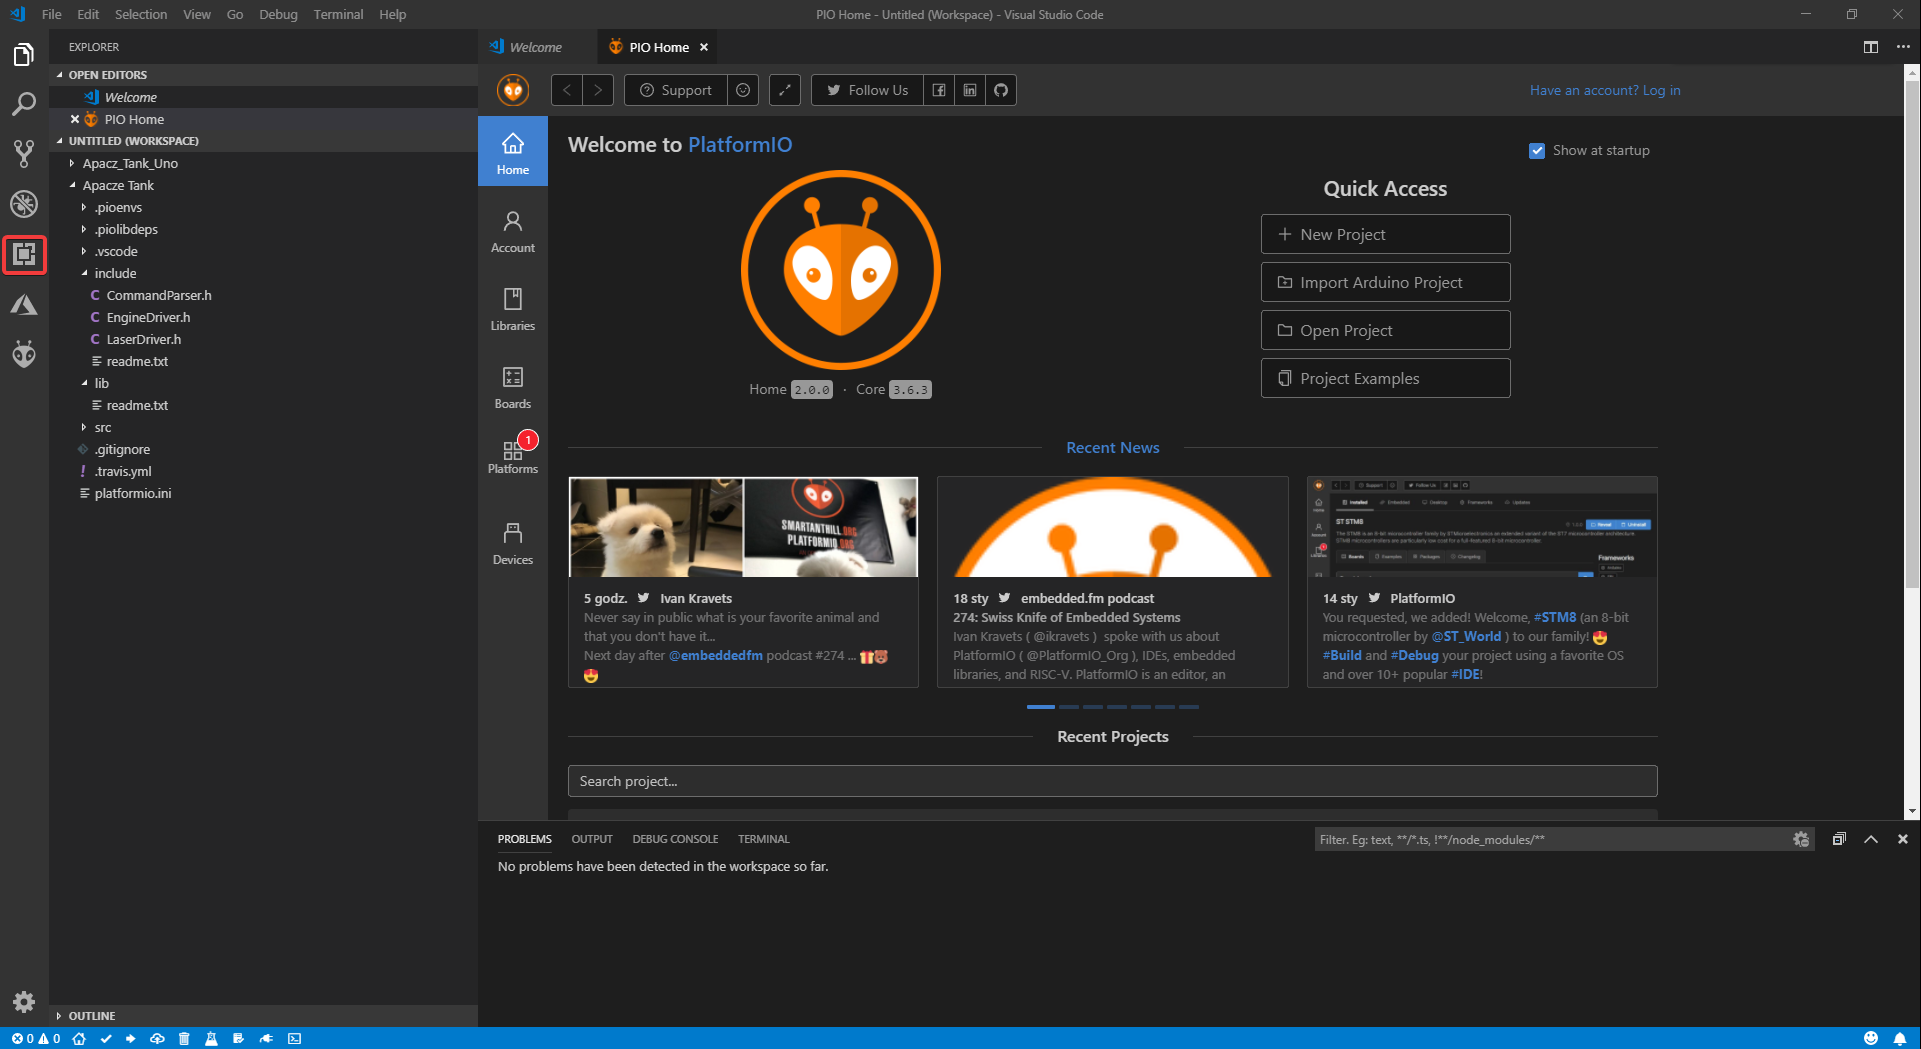
\includegraphics[scale=0.25]{code_1.png}
			\caption{Okno główne edytora Visual Studio Code z zaznaczonym przyciskiem do instalacji rozszerzeń oraz widocznym PlatformIO}
		\end{figure}
	
		Następnie należy wpisać w wyszukiwarkę "Platform IO IDE"  i kliknąć install. 
		
			\begin{figure}[H]
			\centering
			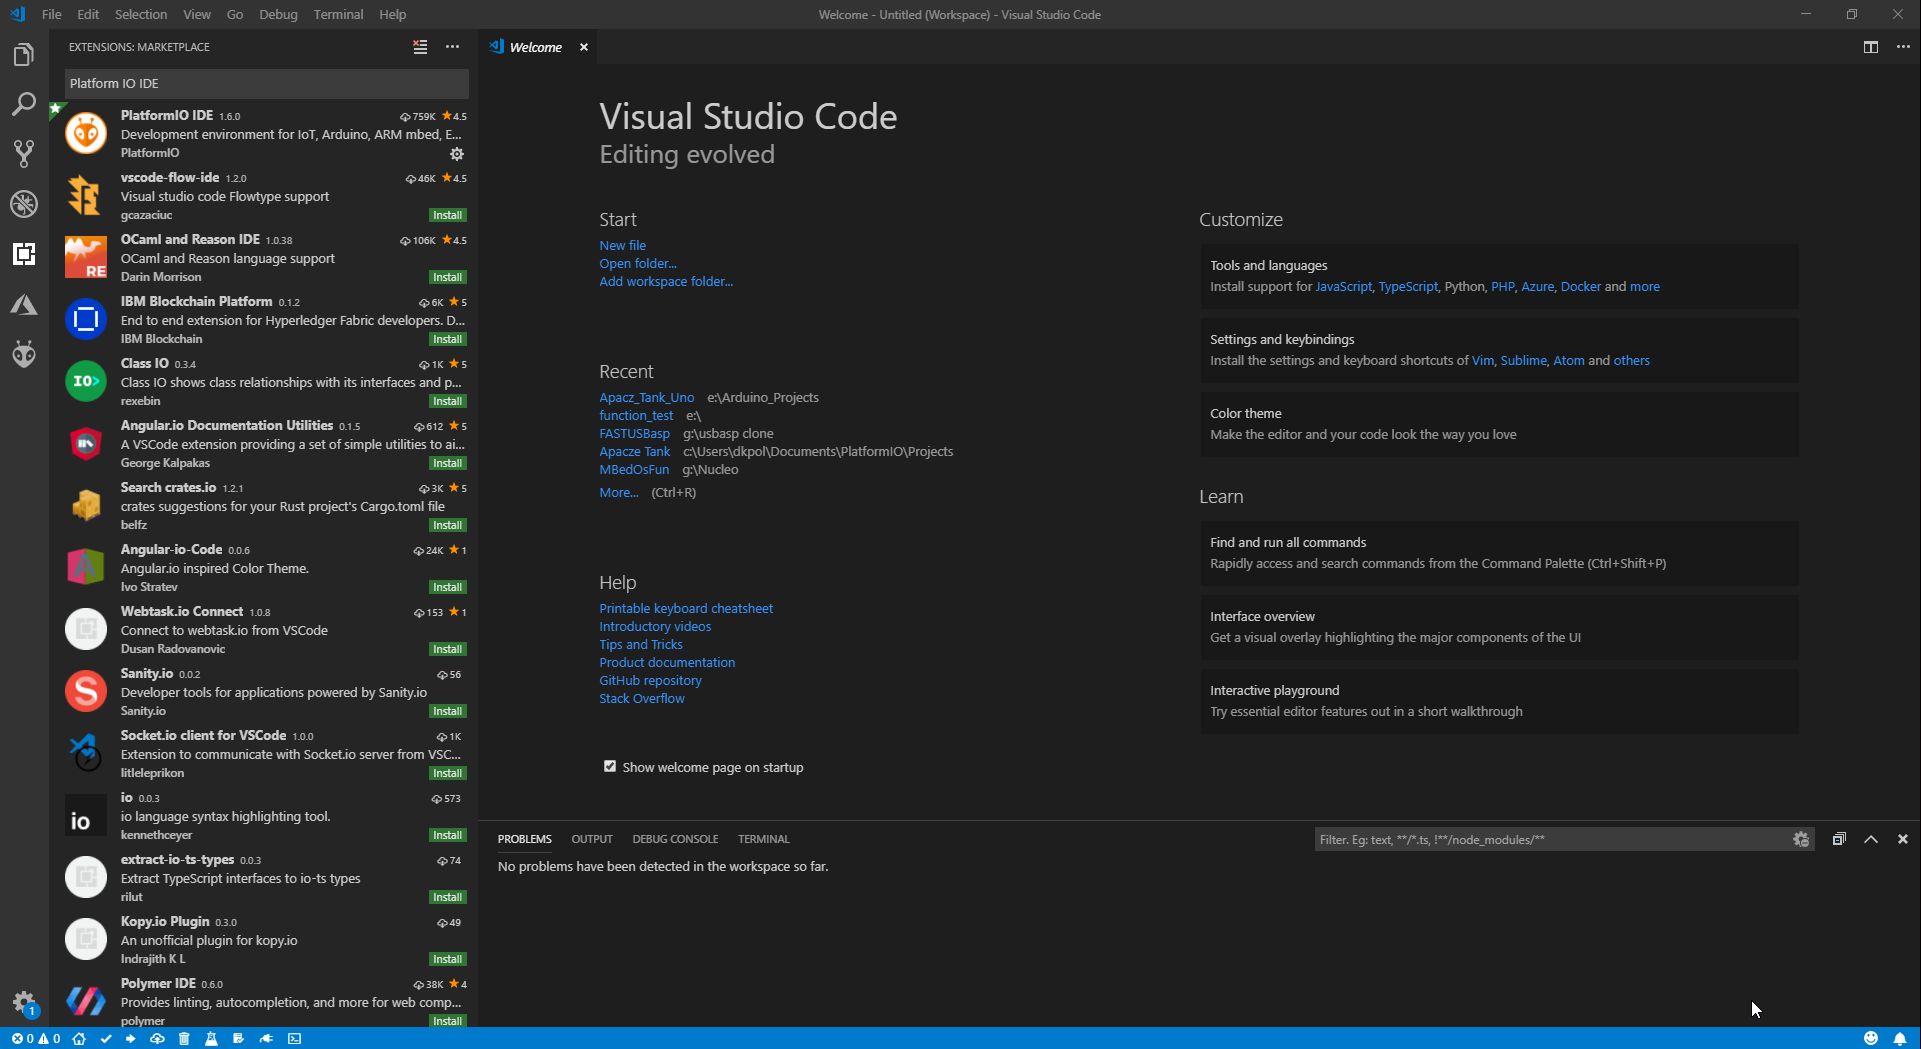
\includegraphics[scale=0.25]{code_2.png}
			\caption{Ekran z włączoną wyszukiwarką rozszerzeń edytora Visual Studio Code}
		\end{figure}
		
    \chapter{Uruchomienie}
        Uruchomienie projektu będzie wymagało wgrania oprogramowania na zgodny telefon z Androidem oraz wgranie firmware do Arduino oraz ustawienia nazwy czołgu przy pomocy poleceń AT
        \section{Android}
	        \subsection{Deploy aplikacji do urządzenia}
	        Uruchom Visual Studio, a następnie otwórz plik projektu Xamarin. (ApaczTank.sln) Po załadowaniu projektu, jeżeli telefon jest podłączony i ma włączony tryb deweloperski z zezwoleniem na debugowanie USB, to powinien być widoczny jako urządzenie testujące. Skompiluj projekt a następnie poczekaj chwilę, aż zostanie on zainstalowany na urządzeniu docelowym.
	        \begin{figure}[H]
	        	\centering
	        	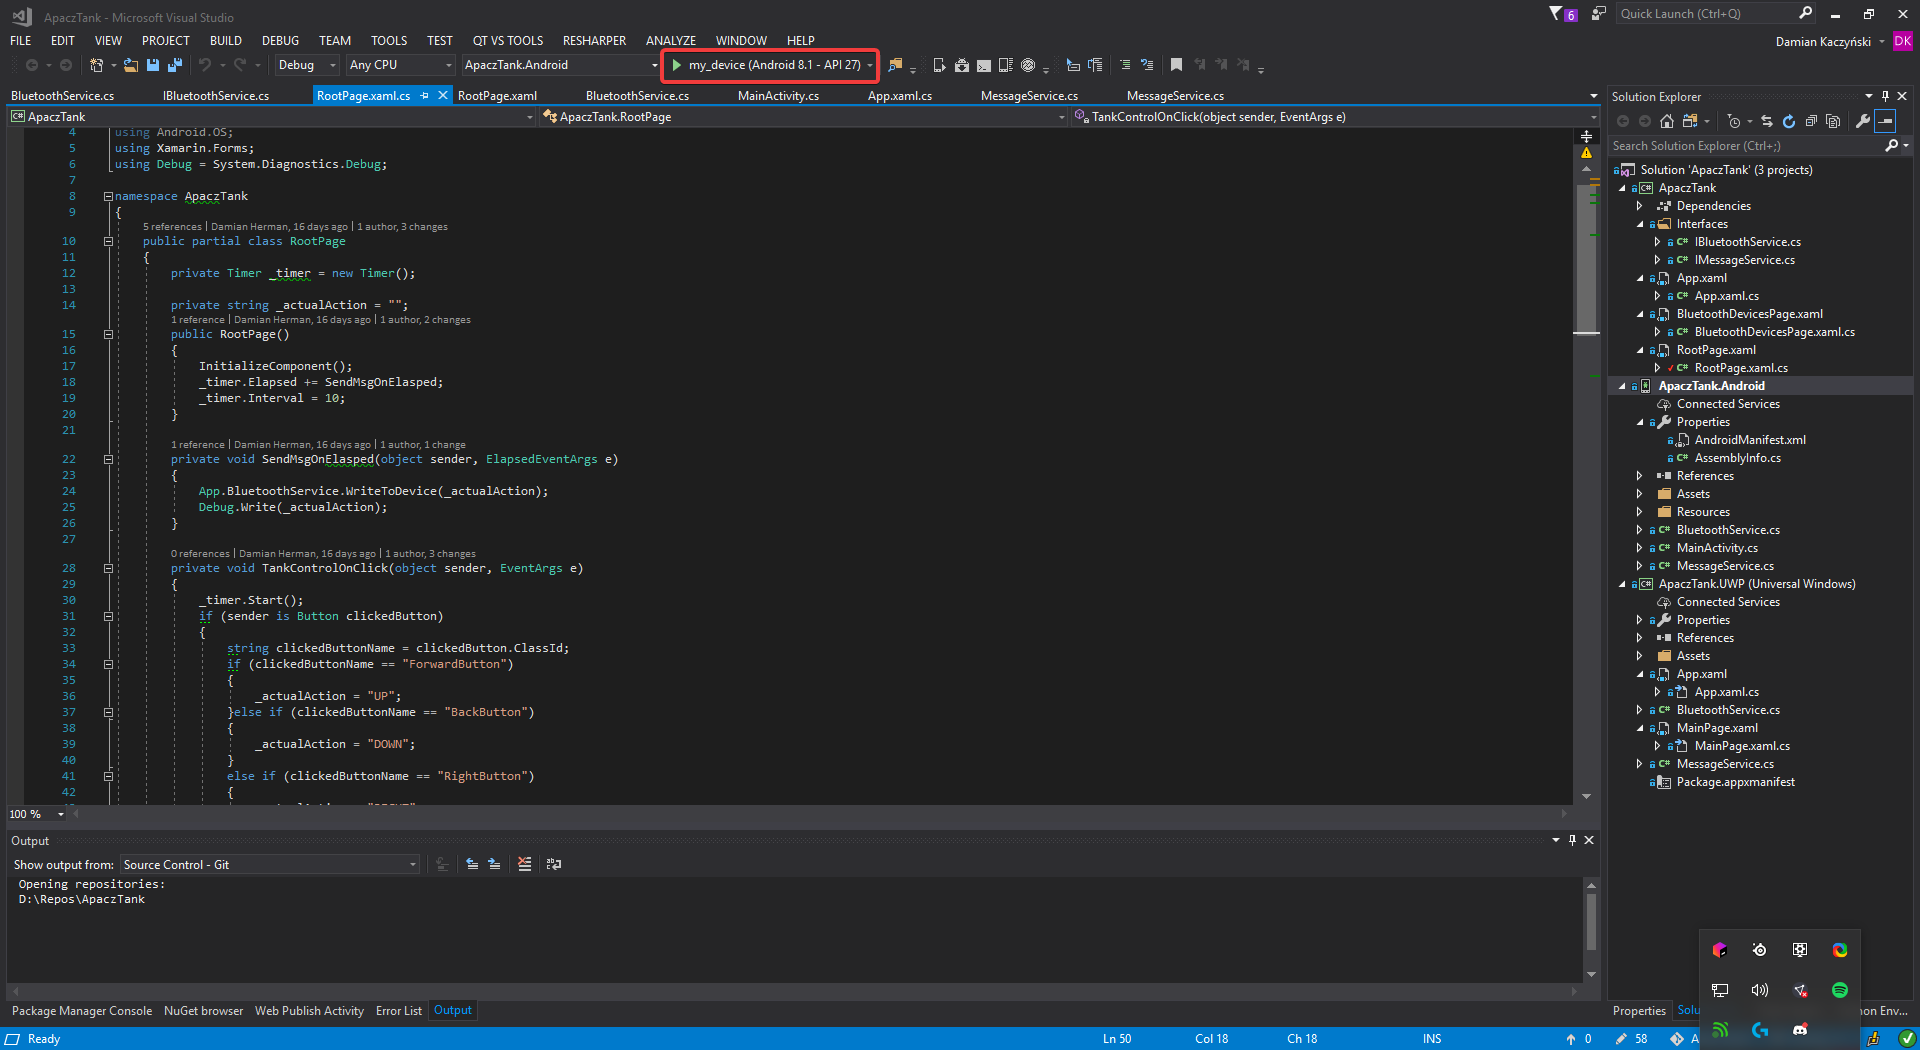
\includegraphics[scale=0.25]{visual_2.png}
	        	\caption{Okno Visual Studio z załadowanym projektem. U góry zaznaczono przycisk kompilacji, zamiast "my
	        		 device"  powinno być urządzenie z Androidem}
	        \end{figure}
	        Aby połączyć się z pojazdem upewnij się, że:
	        \begin{enumerate}
	            \item Bluetooth jest włączony
	            \item Telefon jest sparowany z pojazdem 
	            \item Poczekaj aż niebieska dioda na odbiorniku bluetooth przestanie migać
	        \end{enumerate}
	    	Zakładając poprawną instalację Platform IO, można przystąpić do wgrania firmware do Arduino.
    	\section{Arduino}
	    Otwórz edytor, a następnie kliknij \textit{Open project}. W nowym oknie wybierz lokalizacje projektu i zaakceptuj wybór
	    \begin{figure}[H]
	    	\centering
	    	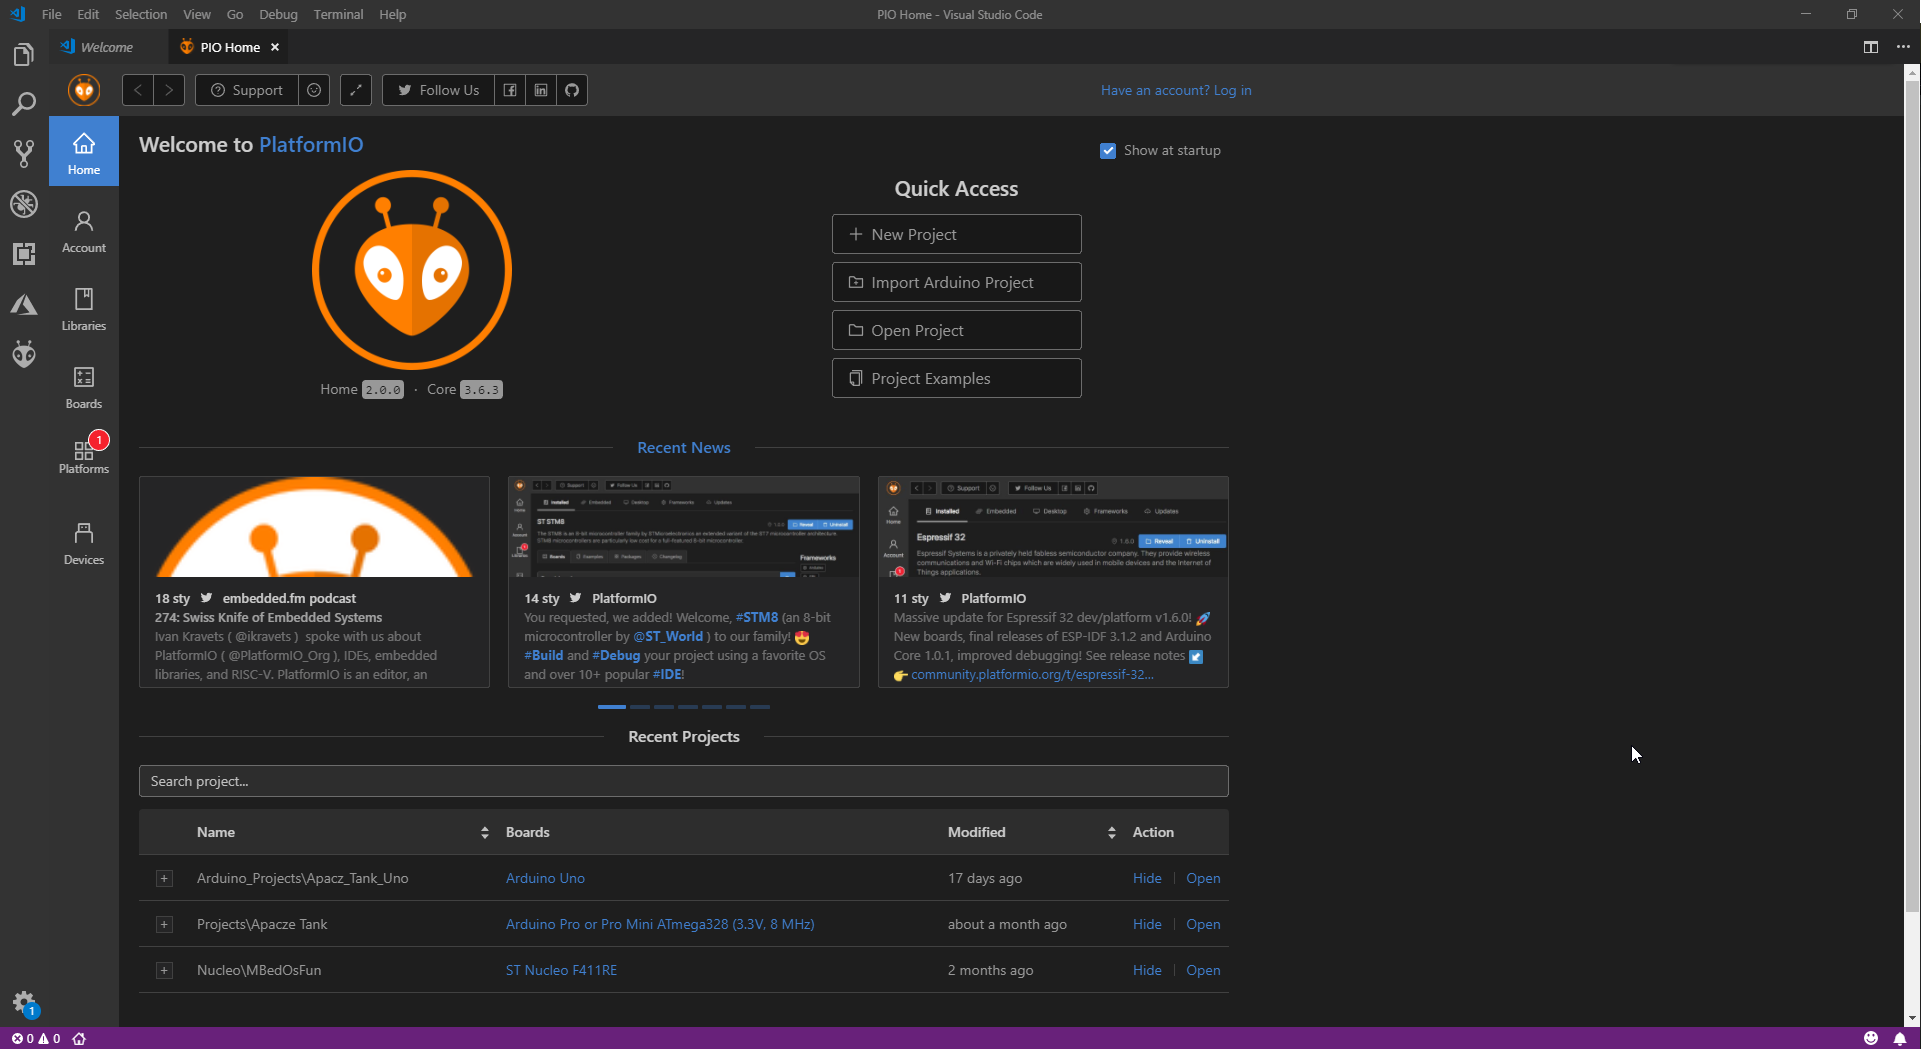
\includegraphics[scale=0.25]{platform_1.png}
	    	\caption{Zrzut ekranowy ekranu powitalnego Platform IO}
	    \end{figure}
	    Po otwarciu projektu naciśnij \textit{PlatformIO: Upload}. Od tego momentu naciskaj przycisk resetu na Arduino Mini Pro, dopóki nie rozpocznie się wgrywanie firmware.
	    \begin{figure}[H]
	    	\centering
	    	
\includegraphics[scale=1]{platform_2.png}
	    	\caption{Pasek narzędziowy środowiska PlatformIO}
	    \end{figure}
    	Jeśli zobaczysz napis \textit{AVRDude done. Thank you.}, to wtedy firmware został wgrany poprawnie.
    \chapter{Opis modułów}
    
    \section{Pojazd}
        \subsection{Mechanika}
        Bazą projektu jest podwozie Dagu Multichassis wyposażony w dwa silniki prądu stałego Dagu DG02S z przekładnią 48:1. 
        \begin{figure}[H]
            \centering
            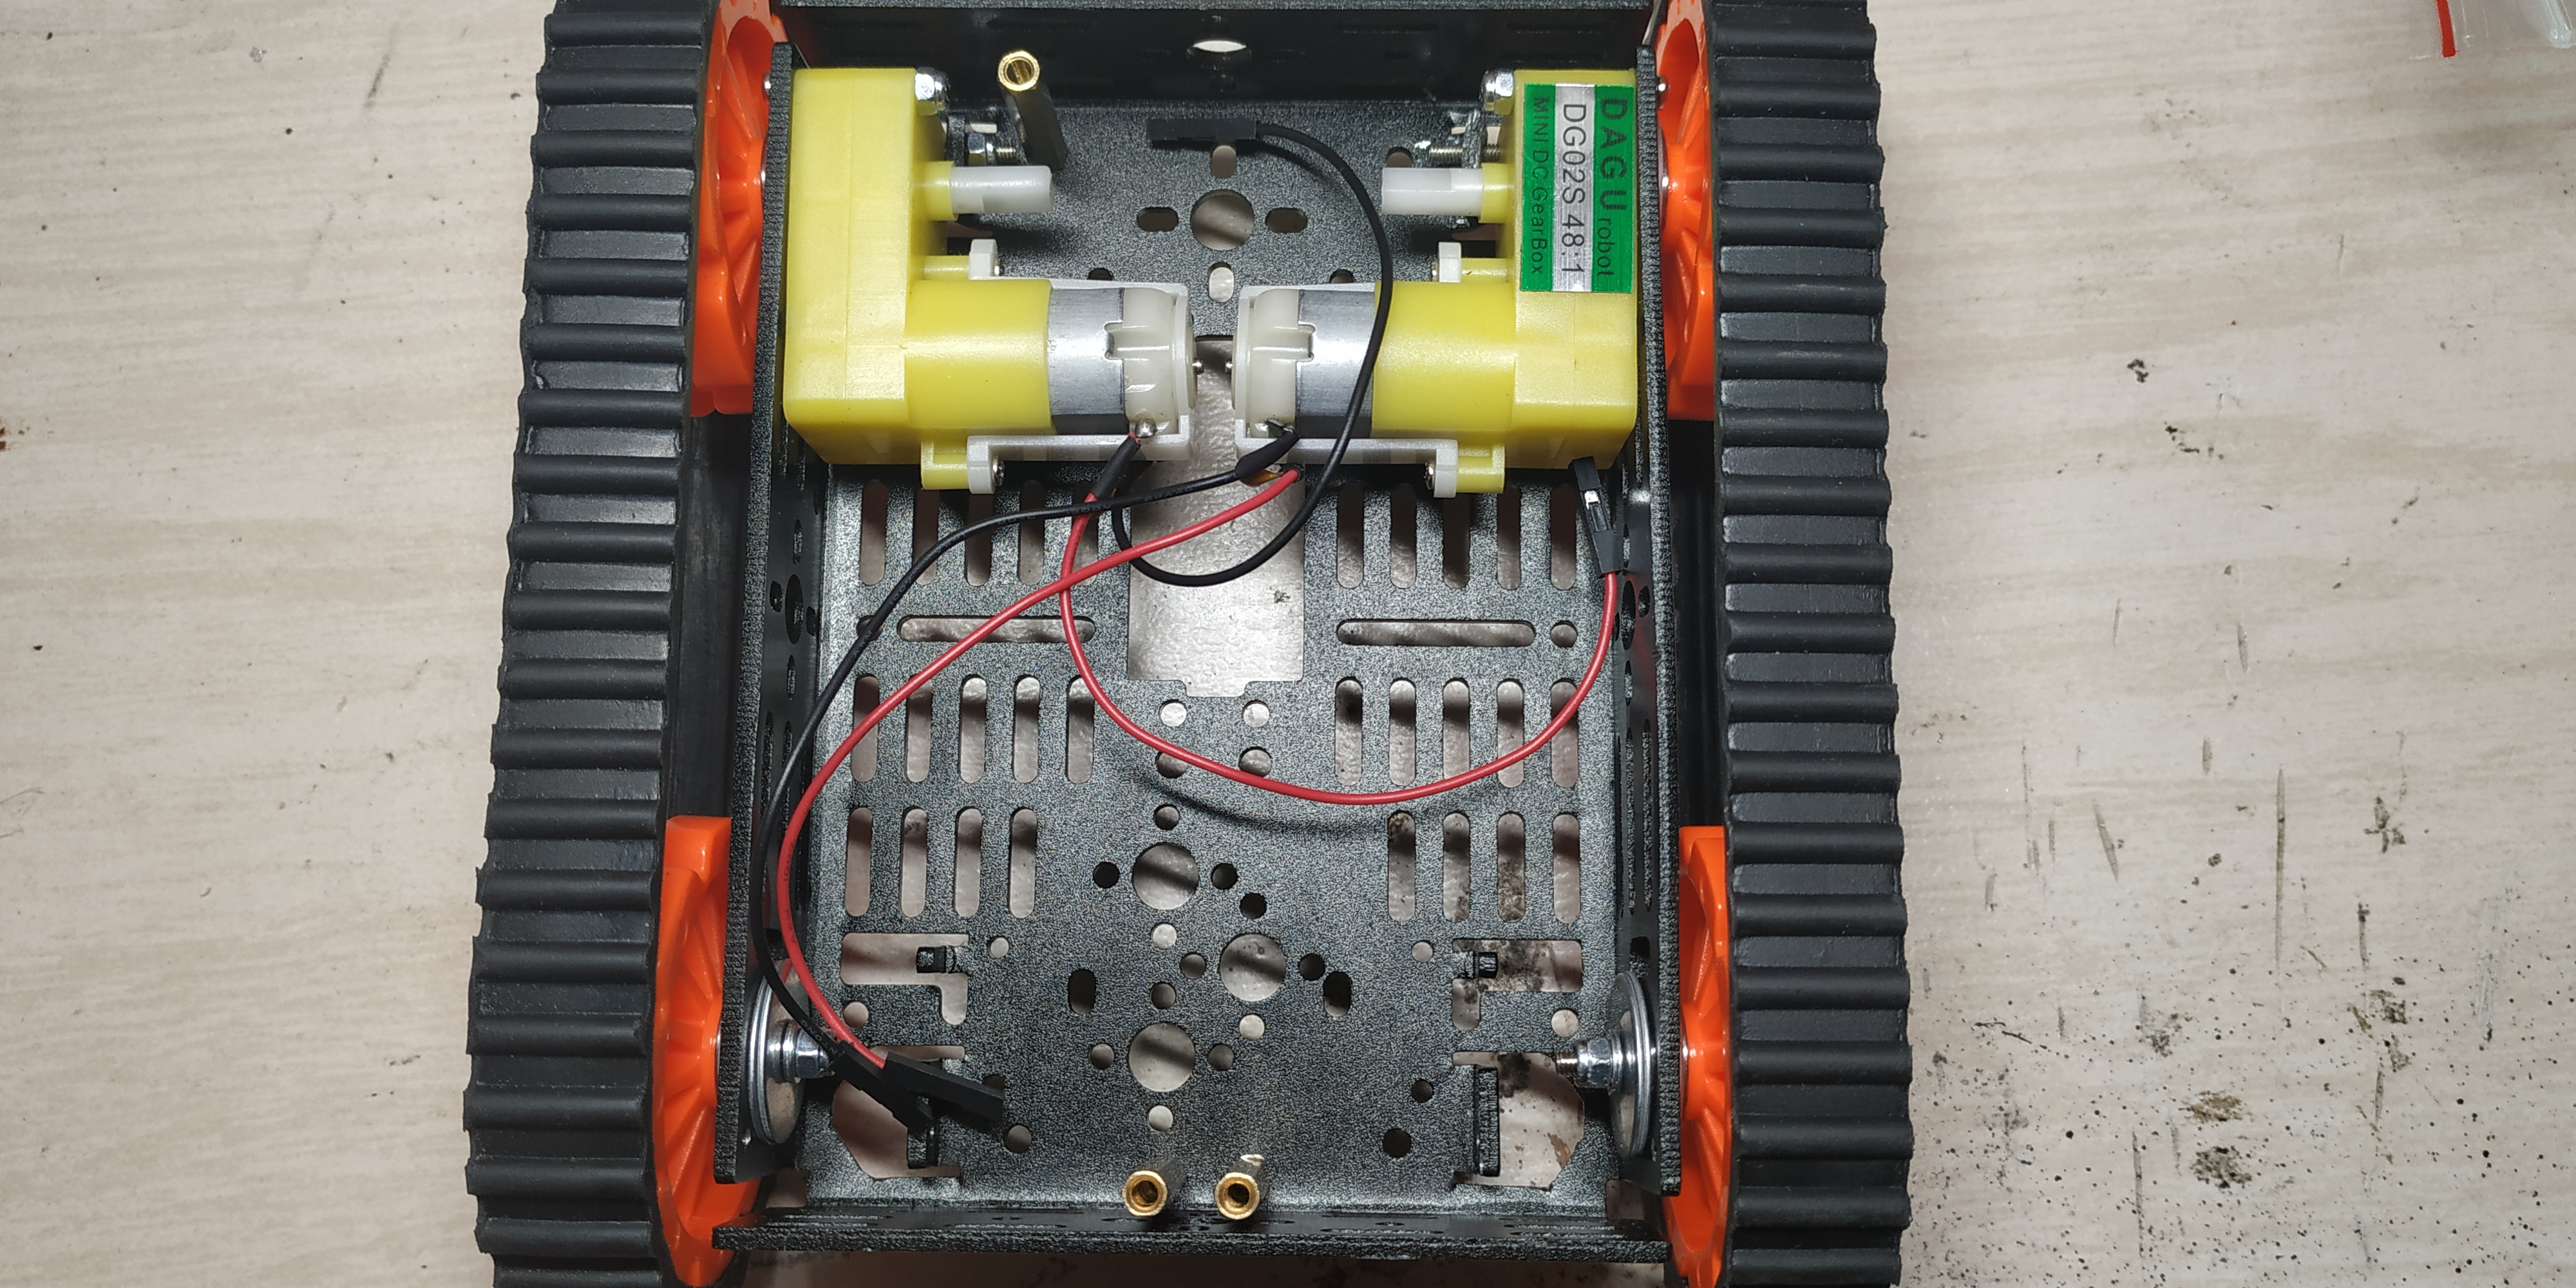
\includegraphics[scale=0.1]{tank_1.jpg}
            \caption{Podwozie pojazdu bez elektroniki}
        \end{figure}
    \section{Elektronika}
        Układ sterujący jest realizowany przy pomocy platformy Arduino, a konkretnie modelu Mini Pro z użyciem zewnętrznego nadajnika-odbiornika Bluetooth HC-05. Za silniki odpowiada układ scalony DRV8835 / L298N.
        Schematy elektroniczne są wykonane za pomocą oprogramowania Autodesk Eagle.
        
       
        \subsection{Zasilanie}
        Projekt jest zasilany akumulatorem Li-Po 2S (7.2V). Pozwala to zmniejszenie masy pojazdu, przy jednoczesnym zwiększeniu prędkości. 
        HC-05 oraz Arduino Mini Pro wymaga zasilania 5V, więc zastosowano liniowy regulator napięcia L7805. 
        \begin{figure}[H]
            \centering
            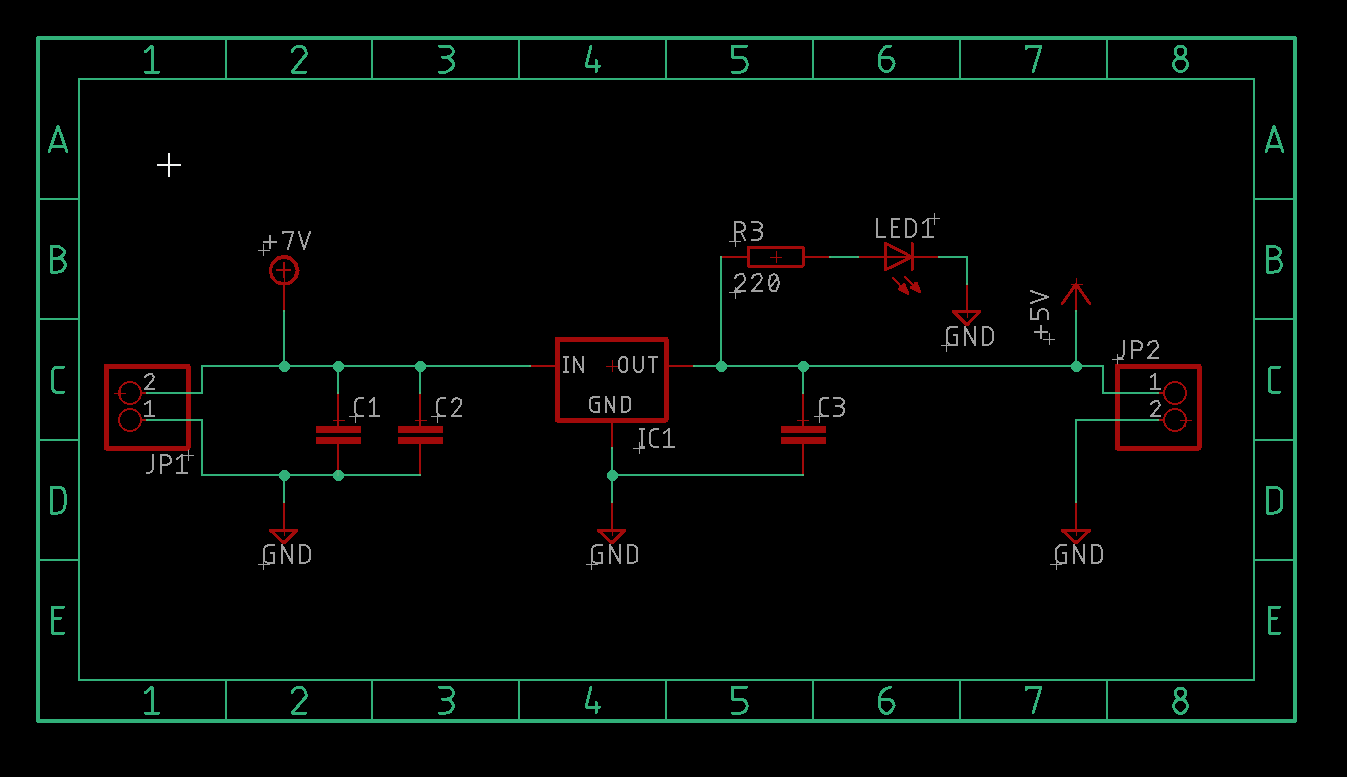
\includegraphics[scale=0.4]{eagle_1.png}
            \caption{Schemat elektroniczny układu zasilającego Arduino Mini Pro oraz HC-05}
        \end{figure} 
    	\subsection{Laser}
		Diodą laserową steruje zwykły tranzystor bipolarny BC337. Prąd lasera to ok. 5mA
        \begin{figure}[H]
			\centering
			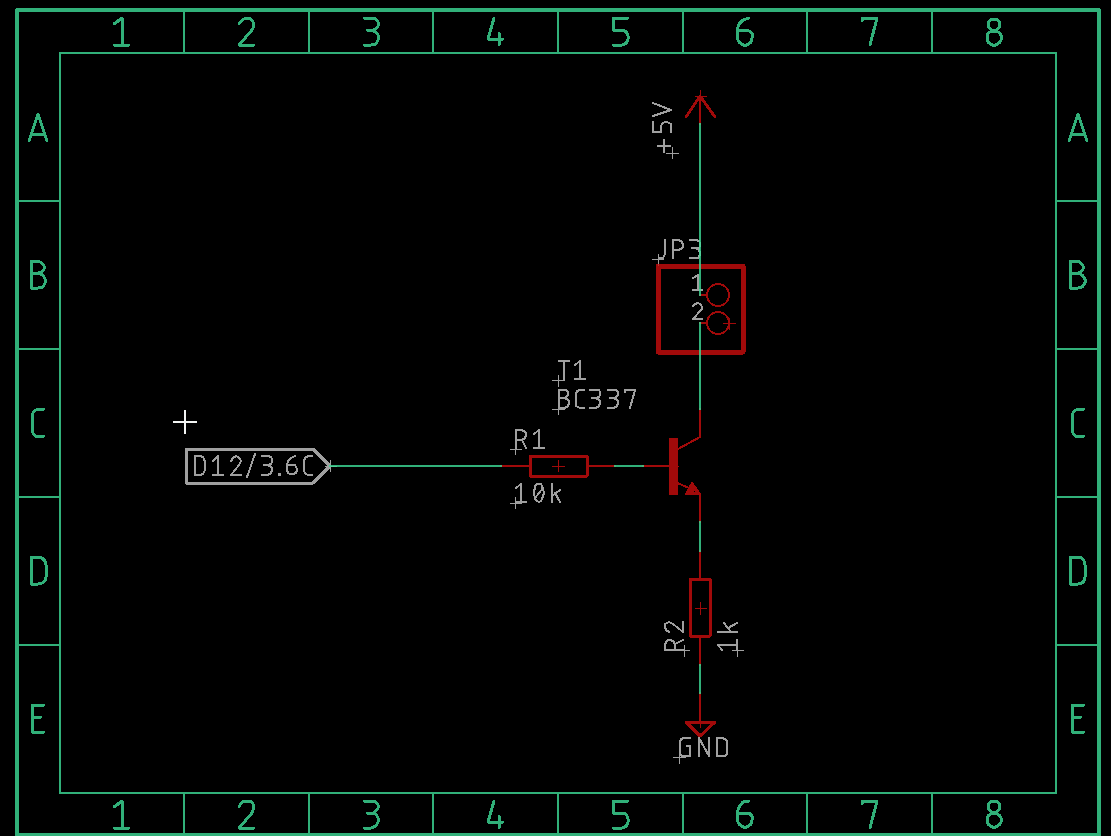
\includegraphics[scale=0.4]{eagle_2.png}
			\caption{Schemat elektroniczny układu sterującego laserem półprzewodnikowym}
		\end{figure}
		\subsection{Płyta główna oraz Bluetooth} 
		Arduino Mini Pro komunikuje się z układem HC-05 przy sprzętowego (programowy \textbf{nie} działa; powstają błędy transmisyjne) układu UART wbudowanego w sam mikrokontroler. Zostały wyprowadzone piny RXI, TX0 do programowania oraz komunikacji z HC-05, GPIO do sterowania sterownikiem silników elektrycznych prądu stałego, GPIO do sterowania laserem, GPIO programowego UART do debugowania kodu.
		 \begin{figure}[H]
			\centering
			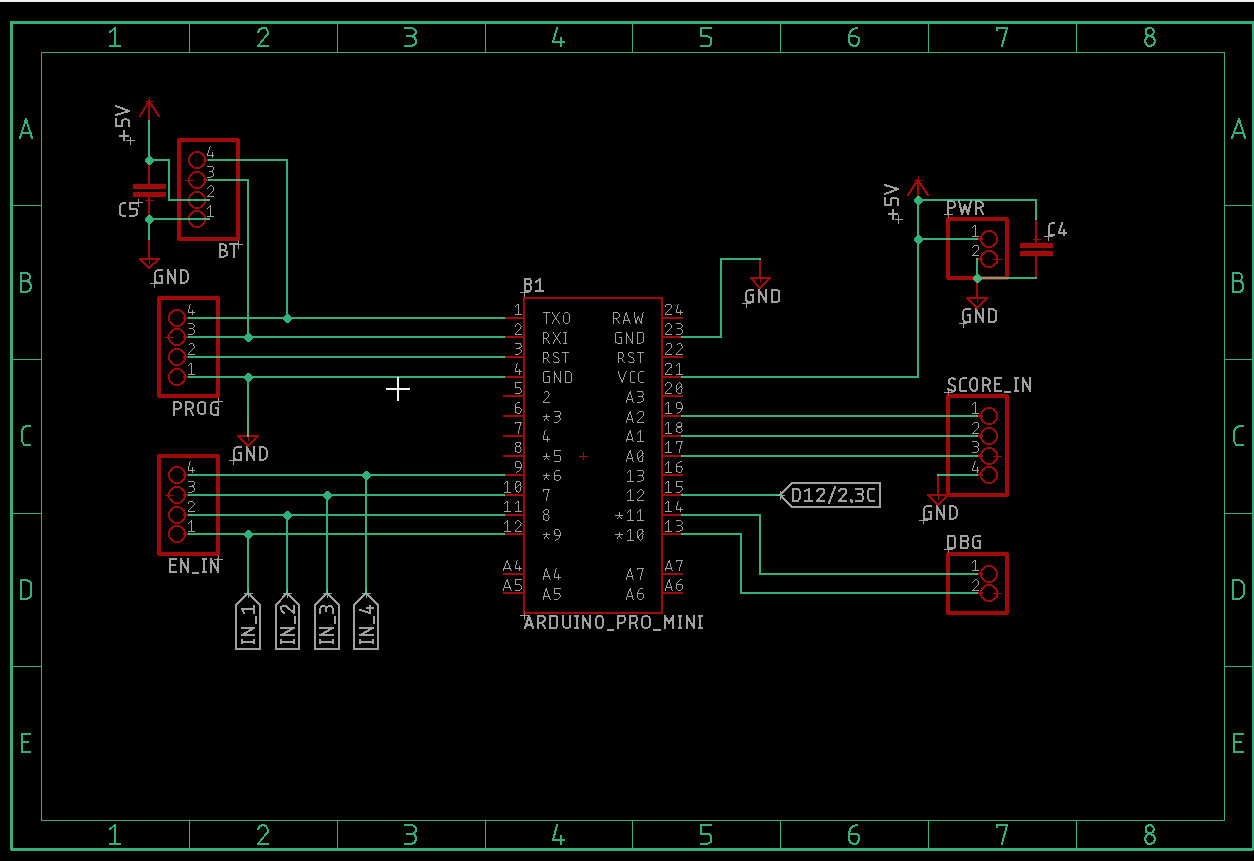
\includegraphics[scale=0.4]{eagle_3.png}
			\caption{Schemat elektroniczny podłączeń do Arduino Mini Pro}
		\end{figure} 
		Na ten moment wszystko jest przylutowane do płytki prototypowej; w planach jest wykonanie obwodu drukowanego.
	    \begin{figure}[H]
			\centering
			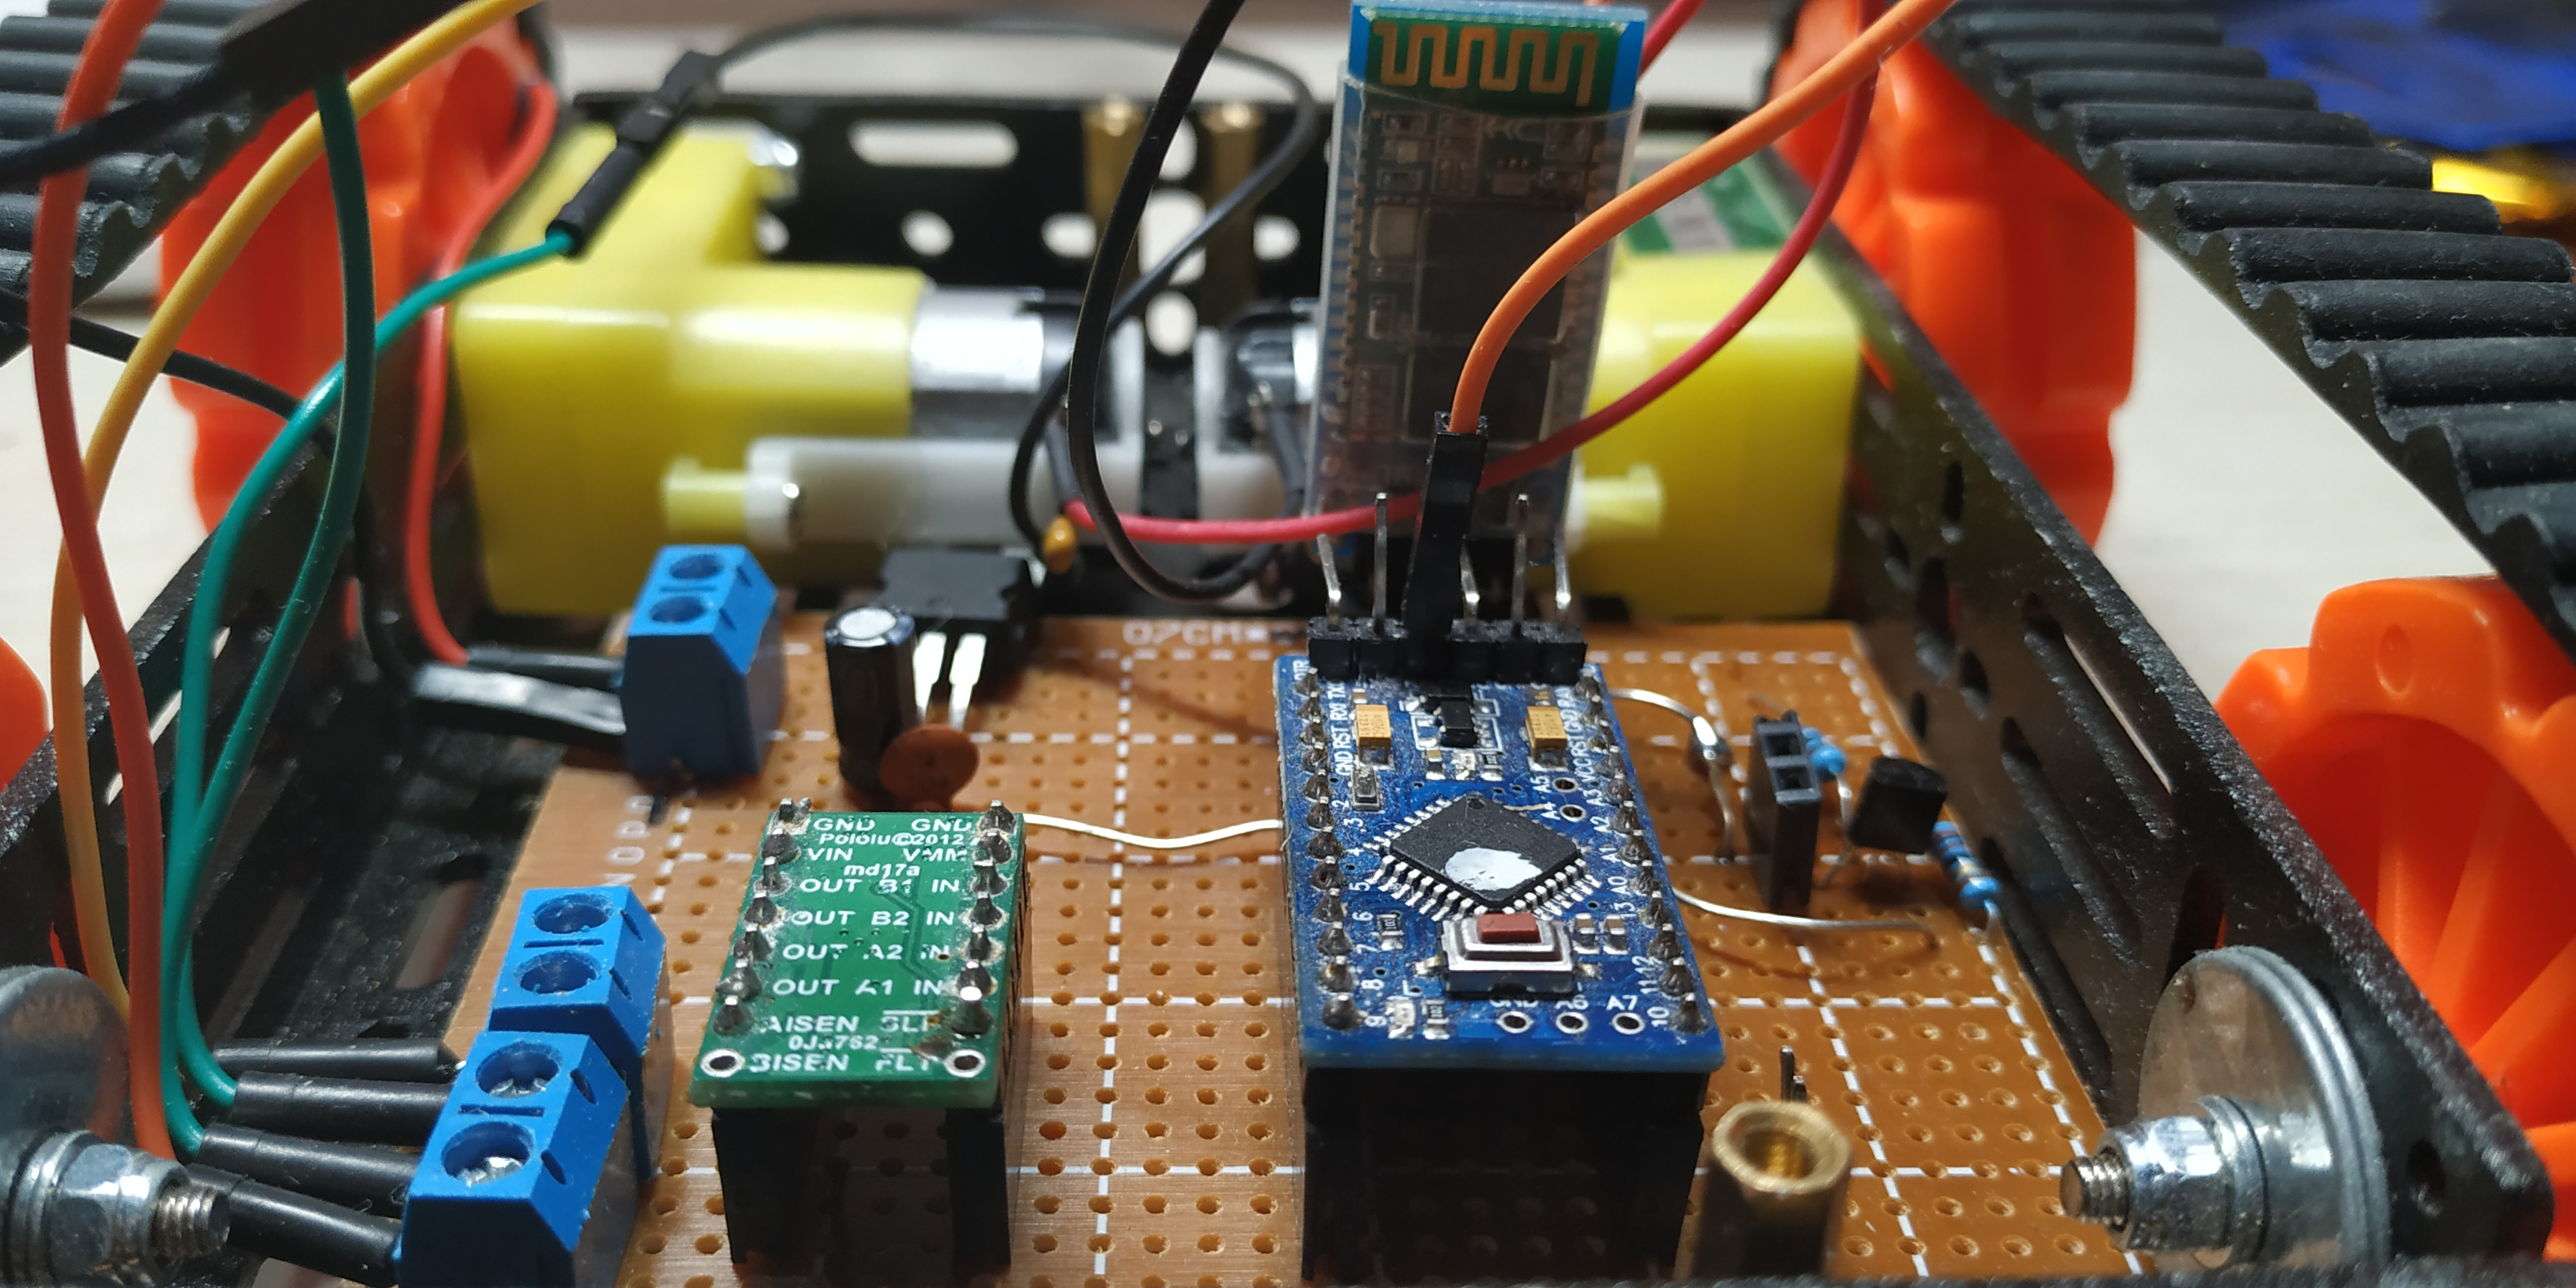
\includegraphics[scale=0.1]{tank_2.jpg}
			\caption{Prototyp głównej płyty głównej projektu. Od lewej: L7805, HC-05, tranzystor BC337 sterujący laserem, DRV8835, Arduino Mini Pro}
		\end{figure}
		\subsection{Punktacja}
		 Za zaliczanie punktacji odpowiadają fotorezystory połączone w dzielnik napięcia, a następnie podłączone do portu ADC. Jeżeli zostanie przekroczona wartość progowa, czołg został trafinony.
		 
	\section{Software}
	Software projektu składa się z kilku części:
	\begin{itemize}
		\item Aplikacja Xamarin do sterowania pojazdem
		\item Firmware pojazdu napisany w oparciu o platformę Arduino
	\end{itemize}
	\subsection{Android.Xamarin}
		GUI aplikacji zostało zaprojektowane, tak aby było jaknajprosztrze. Wykonane zostało w technologii XAML zwalniając dewelopera z definicji układu kontrolek dla każdej z plaform.
		\begin{figure}[H]
			\centering            
			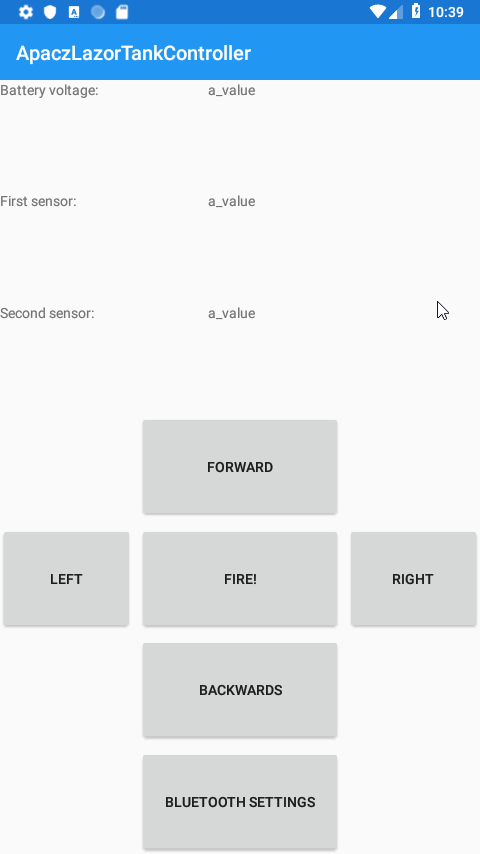
\includegraphics[scale=0.6]{android_1.png}
			\caption{Główny ekran aplikacji, wyświetlający dane z sensorów, kontrolki do sterowania pojazdem oraz przycisk nawigujący do ustawień Bluetooth aplikacji}
		\end{figure}
		\begin{figure}[H]
			\centering            
			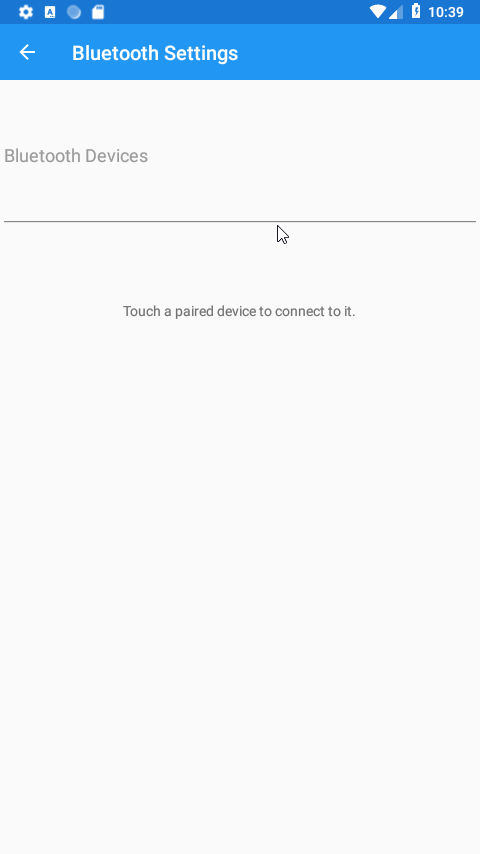
\includegraphics[scale=0.6]{android_2.png}
			\caption{Ekran ustawień Bluetooth, wykrywający czy dane urządzenie wspiera Bluetooth. Po naciśnięciu na listę, zostanie wyświetlona lista sparowanych urządzeń Bluetooth}
		\end{figure}
		W momencie kliknięcia w kontrolkę sterującą, program wysyła co ok. 10 ms komendę do pojazdu docelowego.
	\subsection{Arduino}
	Zasada działania firmware sterującego jest banalne - HC-05 wysyła cokolwiek dostanie na swój port szeregowy. Arduino oczekuje na dane na porcie a następnie odpowiednio porusza silnikami, uruchamia laser.
	Dodatkowo Arduino nasłuchuje na ADC, sprawdzając czy dostał w ścianę. 3 trafienia oznacza unieruchomienie czołgu.
\end{document}
